% Test de refinamiento de colores Weisfeiler-Leman (1-WL)
% Compilar con: pdflatex weisfeiler_leman.tex
\documentclass[tikz,border=10pt]{standalone}
\usepackage{tikz}
\usepackage{amsmath,amssymb}
\usetikzlibrary{arrows.meta, positioning, calc}

\begin{document}
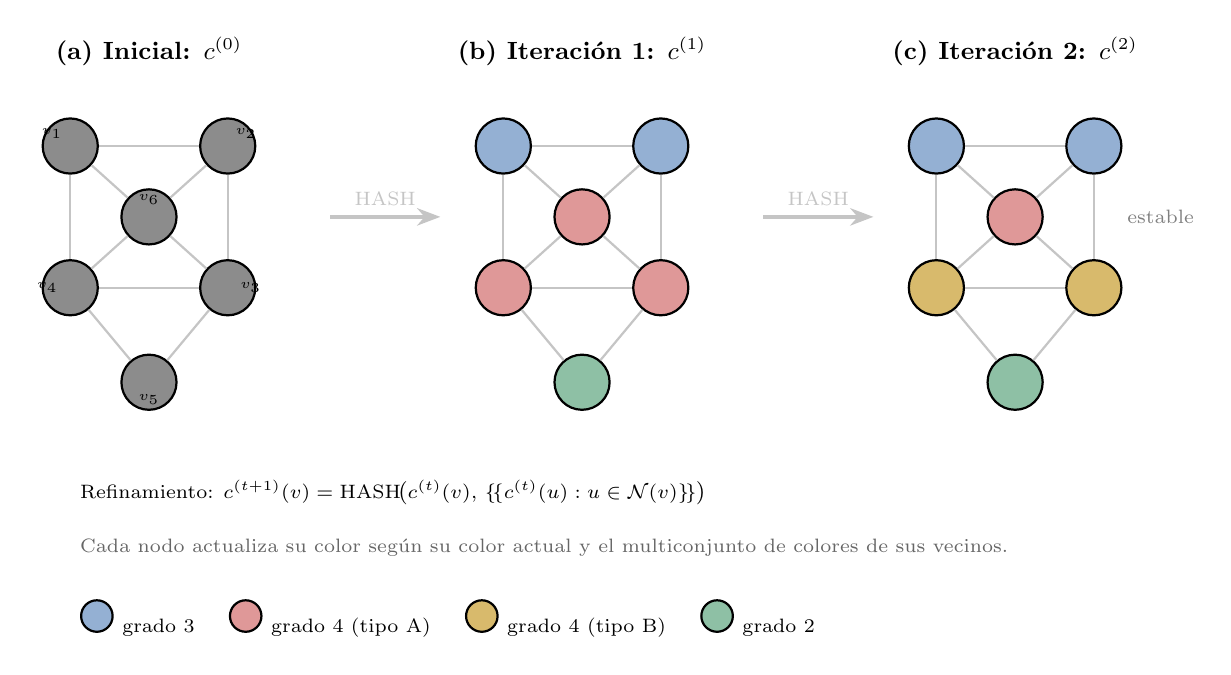
\begin{tikzpicture}[>=Stealth, font=\small,
    wlnode/.style={circle, draw, thick, minimum size=7mm, inner sep=0pt},
    stage/.style={font=\bfseries\small}
]

% Colores
\definecolor{gdlblue}{RGB}{41, 98, 168}
\definecolor{gdlred}{RGB}{191, 49, 49}
\definecolor{gdlgreen}{RGB}{30, 130, 76}
\definecolor{gdlorange}{RGB}{217, 130, 30}
\definecolor{gdlpurple}{RGB}{118, 56, 138}
\definecolor{gdlgray}{RGB}{140, 140, 140}
\definecolor{gdlyellow}{RGB}{190, 140, 10}

% Macro para aristas del grafo (misma topología en las 3 etapas)
\newcommand{\drawedges}{%
    \draw[thick, gdlgray!50] (n1) -- (n2);
    \draw[thick, gdlgray!50] (n2) -- (n3);
    \draw[thick, gdlgray!50] (n3) -- (n4);
    \draw[thick, gdlgray!50] (n4) -- (n1);
    \draw[thick, gdlgray!50] (n3) -- (n5);
    \draw[thick, gdlgray!50] (n4) -- (n5);
    \draw[thick, gdlgray!50] (n1) -- (n6);
    \draw[thick, gdlgray!50] (n2) -- (n6);
    \draw[thick, gdlgray!50] (n3) -- (n6);
    \draw[thick, gdlgray!50] (n4) -- (n6);
}

% Grafo: 6 nodos
% n1--n2, n2--n3, n3--n4, n4--n1 (cuadrado exterior)
% n3--n5, n4--n5 (triángulo inferior)
% n6 conectado a n1,n2,n3,n4 (nodo central)
% Grados: n1=3, n2=3, n3=4, n4=4, n5=2, n6=4

% ============ ETAPA 0: coloración inicial uniforme ============
\begin{scope}[shift={(0,0)}]
    \node[stage] at (1, 3) {(a) Inicial: $c^{(0)}$};
    \node[wlnode, fill=gdlgray] (n1) at (0, 1.8) {};
    \node[wlnode, fill=gdlgray] (n2) at (2, 1.8) {};
    \node[wlnode, fill=gdlgray] (n3) at (2, 0) {};
    \node[wlnode, fill=gdlgray] (n4) at (0, 0) {};
    \node[wlnode, fill=gdlgray] (n5) at (1, -1.2) {};
    \node[wlnode, fill=gdlgray] (n6) at (1, 0.9) {};
    \drawedges
    % Etiquetas de nodos
    \node[font=\tiny, above left=-1pt] at (n1) {$v_1$};
    \node[font=\tiny, above right=-1pt] at (n2) {$v_2$};
    \node[font=\tiny, right=1pt] at (n3) {$v_3$};
    \node[font=\tiny, left=1pt] at (n4) {$v_4$};
    \node[font=\tiny, below=1pt] at (n5) {$v_5$};
    \node[font=\tiny, above=1pt] at (n6) {$v_6$};
\end{scope}

% Flecha
\draw[->, very thick, gdlgray!50] (3.3, 0.9) -- node[above, font=\scriptsize] {HASH} (4.7, 0.9);

% ============ ETAPA 1: refinamiento por grado ============
% n1=3(azul), n2=3(azul), n3=4(rojo), n4=4(rojo), n5=2(verde), n6=4(rojo)
\begin{scope}[shift={(5.5,0)}]
    \node[stage] at (1, 3) {(b) Iteración 1: $c^{(1)}$};
    \node[wlnode, fill=gdlblue!50] (n1) at (0, 1.8) {};
    \node[wlnode, fill=gdlblue!50] (n2) at (2, 1.8) {};
    \node[wlnode, fill=gdlred!50] (n3) at (2, 0) {};
    \node[wlnode, fill=gdlred!50] (n4) at (0, 0) {};
    \node[wlnode, fill=gdlgreen!50] (n5) at (1, -1.2) {};
    \node[wlnode, fill=gdlred!50] (n6) at (1, 0.9) {};
    \drawedges
\end{scope}

% Flecha
\draw[->, very thick, gdlgray!50] (8.8, 0.9) -- node[above, font=\scriptsize] {HASH} (10.2, 0.9);

% ============ ETAPA 2: refinamiento adicional ============
% n3 vecinos: azul,rojo,verde,rojo -> n4 vecinos: azul,rojo,verde,rojo (iguales -> amarillo)
% n6 vecinos: azul,azul,rojo,rojo (diferente de n3,n4 -> sigue rojo)
\begin{scope}[shift={(11,0)}]
    \node[stage] at (1, 3) {(c) Iteración 2: $c^{(2)}$};
    \node[wlnode, fill=gdlblue!50] (n1) at (0, 1.8) {};
    \node[wlnode, fill=gdlblue!50] (n2) at (2, 1.8) {};
    \node[wlnode, fill=gdlyellow!60] (n3) at (2, 0) {};
    \node[wlnode, fill=gdlyellow!60] (n4) at (0, 0) {};
    \node[wlnode, fill=gdlgreen!50] (n5) at (1, -1.2) {};
    \node[wlnode, fill=gdlred!50] (n6) at (1, 0.9) {};
    \drawedges
    % Anotación de convergencia
    \node[font=\scriptsize, text=black!50, anchor=west] at (2.3, 0.9) {estable};
\end{scope}

% === Leyenda inferior ===
\node[anchor=west, font=\scriptsize] at (0, -2.6) {%
    Refinamiento: $c^{(t+1)}(v) = \mathrm{HASH}\!\big(c^{(t)}(v),\, \{\!\{c^{(t)}(u) : u \in \mathcal{N}(v)\}\!\}\big)$};
\node[anchor=west, font=\scriptsize, text=black!60] at (0, -3.3) {%
    Cada nodo actualiza su color según su color actual y el multiconjunto de colores de sus vecinos.};

% Leyenda de colores
\node[anchor=west] at (0, -4.2) {%
    \tikz{\node[wlnode, fill=gdlblue!50, minimum size=4mm] {};} {\scriptsize grado 3} \quad
    \tikz{\node[wlnode, fill=gdlred!50, minimum size=4mm] {};} {\scriptsize grado 4 (tipo A)} \quad
    \tikz{\node[wlnode, fill=gdlyellow!60, minimum size=4mm] {};} {\scriptsize grado 4 (tipo B)} \quad
    \tikz{\node[wlnode, fill=gdlgreen!50, minimum size=4mm] {};} {\scriptsize grado 2}
};

\end{tikzpicture}
\end{document}
